\chapter{Time-Independent Schrodinger Equation}

\section{Exercises}

\exercise{2.1MOD}{
	Prove the following:
	\begin{itemize}
		\item For normalizable solutions, the separation constant E must be real. Hint: take $E = E_0+i\Gamma$, for real constants $\Gamma, E_0$.
		\begin{flalign*}
			\int_{\mathbb{R}}|\Psi|^2~dx&=1\\\\
			\Psi(x,t) &= \psi(x)e^{-\frac{i(E_0+i\Gamma)}{\hbar}t}\\
			|\Psi(x,t)|^2 &= \Psi^*\Psi = \psi^*e^{\frac{iE_0}{\hbar}t}e^{\frac{\Gamma}{\hbar}t}\psi e^{\frac{-iE_0}{\hbar}t}e^{\frac{\Gamma}{\hbar}t}\\
			&= \psi^*\psi e^{\frac{2\Gamma}{\hbar}t} = |\psi(x)|^2 e^{\frac{2\Gamma}{\hbar}t}\\
			\int_{\mathbb{R}}|\Psi|^2~dx &= e^{\frac{2\Gamma}{\hbar}t} \int_{\mathbb{R}}|\psi(x)|^2~dx = 1~\forall t\impliedby e^{\frac{2\Gamma}{\hbar}t} = C \implies \Gamma = 0
		\end{flalign*}
		\item The time-independent wave function $\psi(x)$ can always be taken to be real (unlike $\Psi(x,t)$). This doesn't mean that every solution to the time-ind. Schro equation is real; what it says 
		is that if you've got one that is not, it can always be expressed as a linear combination of solutions (with the same energy) that are. So you might as well stick to $\psi$s that are real.
		\begin{flalign*}
			f(x) &= a+ib, ~a,b \in \mathbb{R}\\
			f(x)+f^*(x) &= 2a \implies a = \frac{f(x)+f^*(x)}{2}\\
			f(x)-f^*(x) &= 2ib\implies b = -i\frac{f(x)-f^*(x)}{2}\\
			-\frac{\hbar^2}{2m}\derivative[2]{\psi}{x}+(V(x)-E)\psi(x) &= 0 = -\frac{\hbar^2}{2m}\derivative[2]{\psi^*}{x}+(V(x)-E)\psi^*(x)\\
		\end{flalign*}
		This last line shows the form for linear, homogeneous ODEs for which their weighted sum also serves as a solution to the original ODE. To get the values for the constants $c$, then we can use $c_1 = c_2 = 1/2$ values for real solutions implied by $a$, or $c_1 = -i/2,~c_2 = i/2$ for real solutions implied by $b$ as well:
		\begin{flalign*}
			f(x) = \psi(x)=c_1\psi(x)+c_2\psi^*(x)
		\end{flalign*}
		If $\psi(x)$ did not have any imaginary term(s), then one would pick any real constants to produce a real solution. Hence, if the solutions for the complex conjugate and the conjugate satisfy the time-ind. Schro for real $E, V(x)$, any linear combination of these will also follow suit. 
		Note that $$\psi = \frac{1}{2}((\psi+\psi^*)+i(-i(\psi-\psi^*)))$$ which shows $\psi$ can be written as a linear combination of two real solutions $\psi+\psi^*$ and $i(\psi-\psi^*)$.  Recall that the complex number system extends the real numbers with the imaginary unit $i$ satisfying $i^2=-1$.
		\item If $V(x)$ is an even function (i.e., $V(-x)=V(x)$), then $\psi(x)$ can always be taken to be either even or odd.
		\begin{flalign*}
			x = -y &\implies -\derivative{y}{x}=1\\
			\derivative{\psi(x)}{x} &= \derivative{\psi(-y)}{(-y)}\cancelto{1}{\derivative{(-y)}{x}}= -\derivative{\psi(-y)}{y}\\
			\derivative[2]{\psi(x)}{x} &= \derivative{}{x}\derivative{\psi}{x} = -\cancelto{1}{\derivative{(-y)}{x}}\derivative{}{(-y)}\derivative{\psi(-y)}{y} = \derivative[2]{\psi(-y)}{y}
		\end{flalign*}
		Now substitute as needed,
		\begin{flalign*}
			-\frac{\hbar^2}{2m}\derivative[2]{\psi(-y)}{(-y)}+(V(-y)-E)\psi(-y) &= -\frac{\hbar^2}{2m}\derivative[2]{\psi(x)}{x}+(V(x)-E)\psi(x)  = 0\\
		\end{flalign*}
		As before, we get a linear ODE for the even-odd pair whose weighted sum also produces a real solution as discussed prior $$\psi(x)=c_1\psi(-x)+c_2\psi(x)$$ Thus, any (real) solution can be expressed as a linear combination of even or odd solutions given an even potential well function with $c_1 = c_2 = 1$ producing a possible even function or $c_1=-1,~c_2=1$ producing a possible odd function, $$f_e=\frac{f(x)+f(-x)}{2},~f_o=\frac{f(x)-f(-x)}{2}$$
		 It's important to note that when dealing with a real physical system, the wave function is generally a complex-valued function. However, the even and odd classifications refer
		 to the symmetry properties of the real part of the wave function. We add the ``wiggle factor'' when including time domain considerations that gets us into imaginary land.\\
		\item Does the prior statement hold for an odd potential function?\\\\
		Here, the probability density of finding the particle is opposite on both sides of the origin. This occurs when the particle's state possesses spatial asymmetry. The statement does not hold for an odd potential well function, where we would strictly need an odd wave function $\psi(x)=-\psi(-x)$ to maintain the proper relation above; an even wave function would contradict the antisymmetric nature of the potential function in this case.  
	\end{itemize}
}

\exercise{2.2}{
	Show that $E$ must exceed the minimum value of $V(x)$, for every normalizable solution to the time-ind Schro. What is the classical analog to this statement?
	
	\begin{equation*}
	-\frac{\hbar^2}{2m}\derivative[2]{\psi}{x}+V(x)\psi=E\psi
	\end{equation*}
			
	Assume that there exists a normalizable solution $\psi(x)$ to the time-independent Schrödinger equation with energy $E$ that satisfies $E < V(x)_{min}$, where $V(x)_{min}$ is the minimum value of the potential energy function $V(x)$. Then we can write:
	
	\begin{equation*}
		E\psi = -\frac{\hbar^2}{2m}\derivative[2]{\psi}{x}+V(x)\psi < V(x)_{min}\psi
	\end{equation*}
	
	Dividing both sides by $\psi$ and rearranging, we get:
	
	\begin{equation*}
	-\frac{\hbar^2}{2m}\derivative[2]{\psi}{x}+(V(x)-V(x)_{min})\psi < 0
	\end{equation*}
	
	Since $\psi$ is normalizable, it must approach zero as $x$ approaches infinity or negative infinity; if we knew the function of $V(x)$ and set $D = V(x)-V(x)_{min}$ and solved for $\psi(x)$, we would get an expression in terms of $x$:
	 

	\begin{flalign*}
		-\frac{\hbar^2}{2m}\derivative[2]{\psi}{x}+D\psi &= k,~k \in \mathbb{R}~(in~Joules,~\psi~dimensionless!)\\
		\psi(x) &= \begin{cases}
			c_1e^{-\frac{\sqrt{2Dm}}{\hbar}x}+c_2e^{\frac{\sqrt{2Dm}}{\hbar}x} & \text{if } k = 0 \impliedby \psi = 0,~E \nless 0 \text{ (see: ZPT, and exception QNEC)} \\
			c_3e^{-\frac{\sqrt{2Dm}}{\hbar}x}+c_4e^{\frac{\sqrt{2Dm}}{\hbar}x}-\frac{|k|}{D} & \text{if } k < 0\\
		\end{cases}
	\end{flalign*}
	 
	 
	Both cases allow us to find constants for the normalization condition to hold. When $x \rightarrow \infty$ then $\psi(x) \rightarrow \infty$. When $x \rightarrow -\infty$ then $\psi(x) \rightarrow -\infty$.
	This implies that any further derivatives have the same sign in these regions. By indicating the negation, we are counteracting the growth of $\psi$ to ``head back'' towards 0, therefore, the negated second derivative term must be zero
	 (when we have non-normalizable $\psi$ = 0, where the probability of finding the system in any particular state is not well-defined) or negative (substituting in $\pm \infty$ always yields a positive second derivative and we need a real solution -- $D>0$ as we shall soon see) for all values of $x$,
	
	\begin{equation*}
	-\frac{\hbar^2}{2m}\derivative[2]{\psi}{x} \leq 0
	\end{equation*}
	
	Combining this with the previous inequality, we get:
	
	\begin{equation*}
	D = (V(x)-V(x)_{min}) < 0
	\end{equation*}
	
	But this contradicts the fact that $V(x)_{min}$ is the minimum value of $V(x)$, which means that $V(x)-V(x)_{min}$ is non-negative for all values of $x$. Also note this would otherwise produce
	 complex-valued solutions to $\psi(x)$. Therefore, our initial assumption that $E < V(x)_{min}$ must be false, and we can conclude that $E$ must meet or exceed the minimum value of $V(x)$ for every normalizable solution to the time-independent Schrödinger equation.

	If the energy is equal to or less than the potential energy at a certain point, the particle would be confined to that region (held by an ``infinite force'') 
	and unable to escape. This situation would violate the classical principle of conservation of energy, which states that the total energy of a system is conserved
	 and cannot be created or destroyed. In this case, the particle would have less energy than the potential energy barrier, and therefore, energy conservation would be
	violated. A more sophisticated analysis can be done by showing this violates the principle of least action: the particle would be in a region where its kinetic energy
	is negative or zero, leading to an imaginary or zero action. However, the principle of least action requires that the action be minimized, which corresponds to a
	 real, non-zero value (proof beyond scope of intro course).\\\\
}

\exercise{2.3}{
	Show that there is no acceptable solution to the (time-ind.) Schro for the infinite square well with $E = 0$ or $E < 0$.
	\begin{flalign*}
		\text{Case where } E &= 0:\\
		\pdv[2]{\psi}{x}&=-\frac{2mE}{\hbar^2}\psi = 0 \implies \psi(x) = Ax+B\\
		\psi(0)&=\psi(a)=0 \implies B = 0 \implies \psi(x) = Ax = 0
	\end{flalign*}
	We get a non-normalizable result $\psi(x) = 0$ whereby any constant of integration becomes a normalization factor, whose simultaneity is nonsensical.
	\begin{flalign*}
		\text{Case where } E < 0:\\
		\pdv[2]{\psi}{x}&=\frac{2mE}{\hbar^2}\psi \implies \psi(x) = Ae^{-\frac{\sqrt{2mE}}{\hbar}x}+Be^{\frac{\sqrt{2mE}}{\hbar}x}\\
		\psi(0)&=0 \implies B = 0 \implies A = -B\\
		\psi(a)&=0,~A=-B \implies B = 0 ~|~\frac{\sqrt{2mE}}{\hbar}x = -\frac{\sqrt{2mE}}{\hbar}x \implies \frac{\sqrt{2mE}}{\hbar} = 0\\
	\end{flalign*}
	In this case all roads lead to having $\psi(x) = 0$ again, which is a non-normalizable solution.
}\\

\exercise{2.4}{
	Calculate $\langle x \rangle,~\langle x^2 \rangle,~\langle p \rangle,~\langle p^2 \rangle,~\sigma_x,~\sigma_p$ for the $n^{th}$ stationary state for the infinite square well. Check that the uncertainty principle is satisfied. Which state comes closest to the uncertainty limit?
	\begin{flalign*}
		\langle x \rangle = \int x|\psi^2|~dx= \frac{2}{a}\int_0^a x\sin^2\bigl(\frac{n\pi x}{a}\bigr)~dx &= \frac{1}{a}\int_0^a x\bigl(1-\cos\bigl(\frac{2n\pi x}{a}\bigr))~dx\\
		&= \frac{1}{a}\int_0^a x-x\cos\bigl(\frac{2n\pi x}{a}\bigr)~dx\\
		&= \frac{a}{2}-\frac{1}{a}\int_0^a x\cos\bigl(\frac{2n\pi x}{a}\bigr)~dx \\
		& = \frac{a}{2}+\cancelto{0}{\frac{x\sin\bigl(\frac{2n\pi x}{a}\bigr)}{2 \pi n}\Biggr|_0^a}-\frac{1}{2 \pi n}\int_0^a \sin \bigl(\frac{2 \pi n x}{a}\bigr)~dx\\
		&= \frac{a}{2} + \frac{a}{4 \pi^2 n^2}\int_0^{2\pi n}\sin(u)~du = \frac{a}{2} + \cancelto{0}{\frac{a}{4 \pi^2 n^2}\cos(u)\Biggr|_0^{2 \pi n}}\\
		&= \frac{a}{2}\\
		\langle x^2 \rangle = \int x^2|\psi^2|~dx= \frac{2}{a}\int_0^a x^2\sin^2\bigl(\frac{n\pi x}{a}\bigr)~dx &= \frac{1}{a}\int_0^a x^2\bigl(1-\cos\bigl(\frac{2n\pi x}{a}\bigr))~dx\\
		&= \frac{1}{a}\int_0^a x^2-x^2\cos\bigl(\frac{2n\pi x}{a}\bigr)~dx\\
		&=\frac{1}{a}\Biggl[\frac{x^3}{3}\Biggr|_0^a - \int_0^a x^2\cos \frac{2 n \pi x}{a}~dx\Biggr] = \frac{1}{a}\Biggl[\frac{a^3}{3} - \frac{a^3}{8n^3\pi^3}\int_0^{2 n \pi} y^2\cos y~dy\Biggr]\\
		&= \frac{1}{a}\Biggl[\frac{a^3}{3} - \frac{a^3}{8n^3\pi^3}\Biggl(\cancelto{0}{y^2\sin y \Biggr|_0^{2 n \pi}} - 2\int_0^{2n\pi}y \sin y ~dy\Biggr)\Biggr]\\
		&= \frac{1}{a}\Biggl[\frac{a^3}{3} - \frac{a^3}{8n^3\pi^3}\Biggl(2y\cos y \Biggr|_0^{2 n \pi}-\cancelto{0}{2 \sin y  \Biggr|_0^{2 n \pi}}\Biggr)\Biggr]\\
		&= \frac{a^2}{3}-\frac{a^2}{2n^2\pi^2} = a^2\Biggl(\frac{1}{3}-\frac{1}{2n^2\pi^2}\Biggr)\\
		\sigma_x = \sqrt{\langle x^2 \rangle - \langle x \rangle^2} &= \frac{a}{2}\sqrt{\frac{1}{3}-\frac{2}{n^2\pi^2}}\\
		\langle p \rangle &= -i\hbar \int_0^a \psi_n^*\pdv{\psi_n}{x}~dx = m\derivative{\langle x \rangle}{t} = 0\\
		\langle p^2 \rangle &= \int_0^a \psi_n^*\Biggl[-i\hbar\derivative{}{x}\Biggr]^2\psi_n~dx = -\hbar^2 \int_0^a \psi_n^* \derivative[2]{\psi_n}{x}~dx\\
		&= \hbar^2 \int_0^a \psi_n^* k^2\psi_n~dx ~~(by~2.24)\\
		&= \frac{2mE_n\hbar^2}{\hbar^2}\int_0^a \psi_n^*\psi_n~dx = 2mE_n = \Biggl(\frac{n \pi \hbar}{a}\Biggr)^2~~(\psi s~orthonormal)\\
		\sigma_p &= \sqrt{\langle p^2 \rangle - \langle p \rangle^2} =\frac{n \pi \hbar}{a}\\
		\sigma_p\sigma_x &= \frac{\hbar}{2}\sqrt{\frac{n^2\pi^2}{3}-2} \geq \frac{\hbar}{2}\\
	\end{flalign*}
	Note that the complex-valued time dependence was ``dropped'' as those terms cancel out. The product is smallest for state $n=1$, $1.136\hbar/2$.
}
\exercise{2.5}{
	A particle in the infinite square well has its initital wave function an even mixture of the first two stationary states: $$\Psi(x,0)=A\Biggl[\psi_1(x)+\psi_2(x)\Biggr]$$ 
	\begin{itemize}
		\item Normalize $\Psi(x,0)$. Recall that, having normalized $\Psi$ at $t = 0$, you can rest assured that it stays normalized -- you can check this explicity after the next item.
			\begin{flalign*}
				1 &= \int \Psi\Psi^*~dx = |A|^2 \int (\psi_1^*+\psi_2^*)(\psi_1+\psi_2)~dx = |A|^2 \int |\psi_1|^2+|\psi_2|^2 +\psi_1^*\psi_2+\psi_2^*\psi_1~dx\\
				&= |A|^2(1+1+0+0)~~(orthonormality)\\
				A &= \frac{1}{\sqrt{2}}\\
				\Psi(x,0)&=\underbrace{\frac{1}{\sqrt{2}}}_{c_n}\Biggl[\psi_1(x)+\psi_2(x)\Biggr]
			\end{flalign*}
		\item Find $\Psi(x,t)$, $|\Psi(x,t)|^2$. Express the latter as a sinusoidal function of time. To simplify, let $\omega = \frac{\pi^2 \hbar}{2ma^2}$.
			\begin{flalign*}
				\Psi(x,t) &= \sum_{n=1}^2 c_n\psi_n e^{-\frac{iE_n}{\hbar}t} = \sum_{n=1}^2 c_n\Psi(x,t) \impliedby \hbar n^2 \omega = E_n\\
				\Psi(x,t) &= \frac{1}{\sqrt{2}}\Biggl[\psi_1(x)e^{-\frac{i \hbar \pi^2}{2ma^2}t}+\psi_2(x)e^{-\frac{4i \hbar \pi^2}{2ma^2}t}\Biggr] = \frac{1}{\sqrt{2}}\Biggl[\psi_1(x)e^{-i \hbar \omega t}+\psi_2(x)e^{-4i \omega t}\Biggr]\\
				&= \frac{1}{\sqrt{2}}\sqrt{\frac{2}{a}}\Biggl(\sin\frac{\pi x}{a} e^{-i\omega t}+\sin \frac{2 \pi x}{a}e^{-4i \omega t}\Biggr) = \frac{e^{-i \omega t}}{\sqrt{a}}\Biggl(\sin \frac{\pi x}{a}+\sin \frac{2 \pi x}{a}e^{-3i \omega t}\Biggr)\\
				|\Psi(x,t)|^2 &= \frac{1}{a}\Biggl(\sin^2 \frac{\pi x}{a}+\sin \frac{2 \pi x}{a}\sin \frac{\pi x}{a}(e^{-3i \omega t}+e^{3 i \omega t})+\sin^2 \frac{2 \pi x}{a}\Biggr)\\
				&= \frac{1}{a}\Biggl(\sin^2 \frac{\pi x}{a} + \sin^2 \frac{2 \pi x }{a} + 2 \sin \frac{\pi x}{a}\sin \frac{2 \pi x}{a}\cos 3\omega t\Biggr)
			\end{flalign*}
		\item Compute $\langle x \rangle$. Notice it oscillates in time. What is the angular frequency of this oscillation? What is the amplitude of oscillation? (If your amplitude is greater than $a/2$, go directly to jail)
			\begin{flalign*}
				\langle x \rangle &= \int x |\Psi|^2 ~dx = \frac{1}{a} \int_0^a x\Biggl(\sin^2 \frac{\pi x}{a} + \sin^2 \frac{2 \pi x }{a} + 2 \sin \frac{\pi x}{a}\sin \frac{2 \pi x}{a}\cos 3\omega t\Biggr)~dx\\
				&= \frac{a}{2}\Biggl(1-\frac{32}{9\pi^2}\cos(3 \omega t)\Biggr)~~(use~trig.~~sum~identities~and~IBP)\\
				Amplitude&:~\frac{a}{2}\frac{32}{9\pi^2}\\
				Angular~Frequency&:~3\omega = 3\frac{E_n}{\hbar n^2} = 3\frac{\pi^2 \hbar}{2 m a^2}
			\end{flalign*}
		\item Compute $\langle p \rangle$.
			\begin{flalign*}
				\langle p \rangle &= m\derivative{\langle x \rangle}{t} = \frac{8 \hbar}{3a}\sin(3 \omega t)
			\end{flalign*}
		\item If you measured the energy of this particle, what values might you get, and what is the probability of getting each of them? Find $\langle H \rangle$. How does it compare with $E_1$ and $E_2$?
			\begin{flalign*}
				\langle H \rangle &= \sum_{n=1}^2 |c_n|^2 E_n = |c_1|^2E_1+|c_2|^2E_2=P_1E_1+P_2E_2 = |1/\sqrt{2}|^2\frac{\pi^2\hbar^2}{2ma^2}+|1/\sqrt{2}|^2\frac{4\pi^2\hbar^2}{2ma^2}  = \frac{1}{2}(E_1+E_2) = \frac{5\pi^2\hbar^2}{4ma^2} 
			\end{flalign*}
			We see that the expectation value of the definite total energy (Hamiltonian) is the average of both excited states in this case.
	\end{itemize}
}

\exercise{2.6}{
	Although the overall phase constant of the wave function is of no physical significance (it cancels out whenever you calculate a measurable quantity), the relative phase of the coefficients of Eqn. 2.17 does matter. For example, suppose we change the relative phase from before:
	$$\Psi(x,0)=A\Biggl[\psi_1(x)+e^{i\phi}\psi_2(x)\Biggr],$$ where $\phi$ is some constant. Find $\Psi(x,t)$, $|\Psi(x,t)|^2$, and $\langle x \rangle$. Study the special case $\phi = \pi/2$ and $\phi = \pi$. Compare with results prior.
	\begin{flalign*}
		A &= \frac{1}{\sqrt{2}}\\
		\Psi(x,t) &= \frac{e^{-i \omega t}}{\sqrt{a}}\Biggl[\sin \frac{\pi x}{a} + \sin \frac{2\pi x }{a} e^{i(\phi-3\omega t)}\Biggr]\\
		|\Psi(x,t)|^2 &= \frac{1}{a}\Biggl[\sin^2 \frac{\pi x}{a} + \sin^2 \frac{2\pi x }{a} + 2 \sin \frac{2\pi x }{a} \sin \frac{\pi x }{a}\cos (3\omega t - \phi)\Biggr]\\
		\langle x \rangle &= \frac{a}{2}\Biggl[1-\frac{32}{9 \pi^2}\cos(3 \omega t - \phi)\Biggr]\\
		\phi = \frac{\pi}{2} &\implies \Psi(x,0) = \frac{1}{\sqrt{2}}\bigl[\psi_1(x)+i\psi_2(x)\bigr]\\
		& \implies \langle x \rangle = \frac{a}{2}\Biggl[1-\frac{32}{9 \pi^2}\sin(3 \omega t)\Biggr]\\
		&\implies \langle x \rangle = \frac{a}{2},~t = 0~(start~time)\\
		\phi = \pi &\implies \Psi(x,0) = \frac{1}{\sqrt{2}}\bigl[\psi_1(x)-\psi_2(x)\bigr]\\
		& \implies \langle x \rangle = \frac{a}{2}\Biggl[1+\frac{32}{9 \pi^2}\cos(3 \omega t)\Biggr]\\
		&\implies \langle x \rangle = \frac{a}{2}\biggl[1+\frac{32}{9 \pi^2}\biggr],~t = 0~(start~time)\\
	\end{flalign*}
	The relative phase of the coefficients $\{c_n\}$ allow us to shift the starting point when measuring the expectation value of position.
}

\exercise{2.7MOD}{
	A particle in an infinite square well has the initial wave function 
	\begin{flalign*}
		\Psi(x,0) = \begin{cases}
			Ax, & 0 \leq x \leq a\\
			A(a-x), & a/2 \leq x \leq a
		\end{cases}
	\end{flalign*}
	\begin{itemize}
		\item Sketch this out and determine normalization constant.
			\begin{flalign*}
				1 &= \int |\Psi|^2~dx = \int \Psi^*\Psi ~dx = |A|^2\Biggl[\int_0^{a/2}x^2~dx + \int_{a/2}^a (a-x)^2~dx\Biggr] \implies A = \frac{2 \sqrt{3}}{\sqrt{a^3}}
			\end{flalign*}
			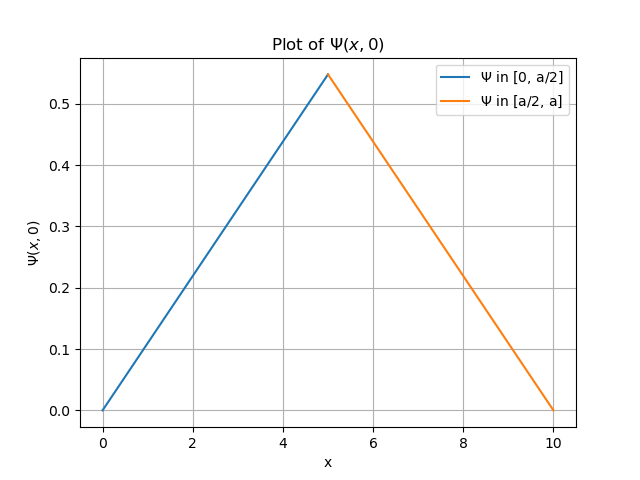
\includegraphics[width=\textwidth]{./chapters/graphs_ch2/2_7_1.png}
		\item Find $\Psi(x,t)$.
			\begin{flalign*}
				\Psi(x,t) =& \sum_{n=1}^\infty c_n\psi_n(x)e^{-\frac{iE_nt}{\hbar}} = \sum_{n=1}^\infty c_n \Psi_n(x,t)\\
				c_n &= \sqrt{\frac{2}{a}}\int_0^a \sin \frac{n \pi x}{a}\Psi(x,0)~dx = \frac{2 \sqrt{3}}{\sqrt{a^3}}\sqrt{\frac{2}{a}} \Biggl[\int_0^{a/2}x\sin \frac{\pi n x}{a}~dx + \int_{a/2}^{a}(a-x)\sin \frac{\pi n x}{a}~dx\Biggr]\\
				&= \frac{4 \sqrt{6}}{n^2\pi^2} \sin \frac{n \pi}{2} = \begin{cases}
					(-1)^{\frac{n-1}{2}}\frac{4 \sqrt{6}}{n^2\pi^2}, & n \text{ odd}\\
					0, & n \text{ even}
				\end{cases}\\
				\therefore \Psi(x,t) &= \frac{4 \sqrt{6}}{\pi^2} \sqrt{\frac{2}{a}} \sum_{1,3,5,\ldots} \frac{(-1)^{\frac{n-1}{2}}}{n^2}\sin \frac{n \pi x}{a}e^{-\frac{iE_nt}{\hbar}}\\
				E_n &= \frac{n^2\pi^2\hbar^2}{2ma^2}
			\end{flalign*}
		\item What is the probability that the measurement of the energy would yield a value $E_1$?
			\begin{flalign*}
				|c_1|^2 = 0.9855
			\end{flalign*}
		\item Find the expectation value of the energy, using Eqn. 2.21.
			\begin{equation*}
				\langle H \rangle = \sum_{n=1,3,5,\ldots}^\infty |c_n|^2E_n = \frac{96\hbar^2}{2ma^2 \pi^2}\Biggl(\frac{1}{1^2}+\frac{1}{3^2}+\frac{1}{5^2}+\ldots\Biggr) = \frac{96\hbar^2}{2ma^2 \pi^2}\underbrace{(1-2^{-2})\zeta(2)}_{\frac{\pi^2}{8}} = \frac{6 \hbar^2}{ma^2} 
			\end{equation*}
		\item Determine how the Fourier Transform, Riemann's Zeta Function, and Basel problem are related.
		\\\\Consider the Basel problem. We can express a function using the Fourier Transform. Consider the function $x^2$ that is continuos and differentiable on $[-L,L]=[-\pi, \pi]$.\\
		\begin{flalign*}
			f(x) &= \frac{a_0}{2}+\sum_{n=1}^{\infty}\Biggl(a_n\cos\frac{n \pi x }{L}+b_n\sin\frac{n \pi x }{L}\Biggr)\\
			\frac{a_0}{2} &= \frac{1}{2L}\int_{-L}^Lf(x)~dx = \frac{2}{2 \pi} \int_0^\pi x^2~dx = \frac{\pi^2}{3}\\
			a_n &= \frac{1}{L} \int_{-L}^{L} f(x) \cos \frac{n \pi x}{L}~dx = \frac{2}{\pi} \int_0^\pi x^2 \cos(n x) ~dx = \frac{4}{n^2}(-1)^n\\
			b_n &= \frac{1}{L} \int_{-L}^{L} f(x) \sin \frac{n \pi x}{L}~dx = \frac{1}{\pi} \int_{-\pi}^\pi x^2 \sin(n x) ~dx = 0\\
			f(\pi) = \pi^2 &= \frac{\pi^2}{3} + \sum_{n=1}^{\infty} \frac{4(-1)^n}{n^2}\cancelto{(-1)^n}{\cos(\pi n)} \iff 4 \sum_{n=1}^{\infty}\frac{1}{n^2}= \frac{2 \pi^2}{3} \implies \sum_{n=1}^{\infty}\frac{1}{n^2} = \frac{\pi^2}{6} \\
			f(0) = 0 &= \frac{\pi^2}{3} + \sum_{n=1}^{\infty} \frac{4(-1)^n}{n^2}\cancelto{1}{\cos(0)} \iff - \sum_{n=1}^{\infty}\frac{(-1)^n}{n^2} = \sum_{n=1}^{\infty}\frac{(-1)^{n+1}}{n^2} = \frac{\pi^2}{12}\\
		\end{flalign*}
		The last two last lines are two such ``problems'' and note how we can take different functions to determine coefficients which the below will also show. Euler did the above differently (see YouTube) but now we can turn to Riemann's Zeta Function.
		\begin{flalign*}
			\frac{\pi^2}{6} &= \frac{1}{1^2}+\frac{1}{2^2}+\frac{1}{3^2}+\ldots\\
			\frac{1}{2^2}\frac{\pi^2}{6} &= \frac{1}{2^2}+\frac{1}{4^2}+\frac{1}{6^2}+\ldots\\
			(1-\frac{1}{2^2})\frac{\pi^2}{6} &= \frac{1}{1^2}+\frac{1}{3^2}+\frac{1}{5^2}+\ldots =\frac{\pi^2}{8}\\
			(1-\frac{2}{2^2})\frac{\pi^2}{6} &= \frac{1}{1^2}-\frac{1}{2^2}+\frac{1}{3^2}-\frac{1}{4^2}+\ldots=\frac{\pi^2}{12}\\
		\end{flalign*}
		Now, generalize.
		\begin{flalign*}
			\zeta(z) = \frac{\pi^2}{6} &= \frac{1}{1^z}+\frac{1}{2^z}+\frac{1}{3^z}+\ldots\\
			(1-\frac{1}{2^z})\zeta(z) &= \frac{1}{1^z}+\frac{1}{3^z}+\frac{1}{5^z}+\ldots\\
			\frac{1}{2^z}\zeta(z) &= \frac{1}{2^z}+\frac{1}{4^z}+\frac{1}{6^z}+\ldots\\
			(1-\frac{2}{2^z})\frac{\pi^2}{6} &= \frac{1}{1^z}-\frac{1}{2^z}+\frac{1}{3^z}-\frac{1}{4^z}+\ldots\\
		\end{flalign*}
		Note for the harmonic series case, we may assume it converges. With this in mind, the second line below produces a greater sum, which we assume also converges. But, the sum of this line must be the sum of the last line, which is greater still. Thus, our initial assumption was wrong and all of them must diverge.
		\begin{flalign*}
			\zeta(1) &= \frac{1}{1}+\frac{1}{2}+\frac{1}{3}+\ldots = \infty\\
			(1-0.5)\zeta(1) &= \frac{1}{1}+\frac{1}{3}+\frac{1}{5}+\ldots = 0.5 \zeta(1) = \infty\\
			0.5 \zeta(1) &= \frac{1}{2}+\frac{1}{4} +\frac{1}{6}+\ldots = \infty\\
		\end{flalign*}
		\item Discuss the general equation for the Riemann zeta function at even integers.\\\\
		The equation for the Riemann zeta function at even integers can be stated as follows:

		For any positive even integer \(s\), where \(s = 2k\) for some positive integer \(k\), the Riemann zeta function \(\zeta(s)\) is given by:

		\[\zeta(2k) = \frac{(-1)^{k+1} \cdot (2\pi)^{2k} \cdot B_{2k}}{2 \cdot (2k)!},\]

		where \(\pi\) is the mathematical constant pi, \(B_{2k}\) is the \(2k\)th Bernoulli number, and \((2k)!\) is the factorial of \(2k\).

		One common definition of the Bernoulli numbers is through their generating function:

		\[
		\frac{t}{e^t - 1} = \sum_{n=0}^{\infty} \frac{B_n}{n!} t^n,
		\]

		where \(B_n\) represents the \(n\)th Bernoulli number.

		Another way to define the Bernoulli numbers is using the recursive formula:

		\[
		B_0 = 1, \quad \text{and} \quad B_n = -\frac{1}{n+1} \sum_{k=0}^{n-1} \binom{n+1}{k} B_k,
		\]

		where \(\binom{n+1}{k}\) denotes the binomial coefficient, which is the number of ways to choose \(k\) objects from a set of \(n+1\) objects.

		These definitions allow us to compute the Bernoulli numbers for any given index \(n\). However, it's worth noting that for odd indices \(n\) greater than 1, the Bernoulli numbers are always equal to zero.			
		In summary, the Riemann zeta function at even integers is expressed in terms of the Bernoulli numbers and the constant \(\pi\), providing a closed-form formula for these specific values of \(s\). No closed-form expression yet exists for odd positive integers of the Ziemann function.
	\end{itemize}
}

\exercise{2.8}{
	A particle of mass $m$ in the infinite square well (of width $a$) starts out in the state $$\Psi(x,0) = \begin{cases}
		A, & 0 \leq x \leq a/2\\
		0, & a/2 \leq x \leq a
	\end{cases}$$ for some constant $A$, so it is (at $t=0$) equally likely to be found at any point in the left half of the well. What is the probability that a measurement of the energy
	at some later time would yield the value of $\frac{\hbar^2 \pi^2}{2ma^2}$?
	\begin{flalign*}
		1 &= \int \Psi\Psi^*~dx = |A|^2 \int_0^{a/2}~dx \implies A = \sqrt{\frac{2}{a}}\\
		E_n &= \frac{\hbar^2 \pi^2 n^2}{2ma^2} \implies E_1 = \frac{\hbar^2 \pi^2}{2ma^2} \impliedby n=1\\
		c_n &= \sqrt{\frac{2}{a}} \int_0^a \sin \frac{\pi x n}{a}\Psi(x,0)~dx = \sqrt{\frac{2}{a}}\sqrt{\frac{2}{a}} \int_{0}^{a/2} \sin \frac{\pi n x}{a} ~dx = -\frac{2}{\pi}(\cos \frac{\pi n}{2}-1)\\
		c_1 & = \frac{2}{\pi} \implies P_1 = |c_1|^2 = 0.4053
	\end{flalign*}
}
\exercise{2.9}{
	For the wave function in Example 2.2, find the expectation value of $H$, at time $t=0$, the old-fashioned way: $$\langle H \rangle = \int \Psi(x,0)^*\hat{H}\Psi(x,0)~dx$$  Compare this result to that of Example 2.3. Because $\langle H \rangle $ is time-ind. then no loss of generality in using this time.
	\begin{flalign*}
		\langle H \rangle &= \int \Psi(x,0)^*\hat{H}\Psi(x,0)~dx\\
		&=\int_0^a \biggl[\sqrt{\frac{30}{a^5}}x(a-x)\biggr]^*\Biggl[-\frac{\hbar}{2m}\pdv[2]{}{x}+\cancelto{0}{V(x)}\Biggr]\biggl[\sqrt{\frac{30}{a^5}}x(a-x)\biggr]~dx\\
		&=\int_0^a \biggl[\sqrt{\frac{30}{a^5}}x(a-x)\biggr]\Biggl[-\frac{\hbar}{2m}\pdv[2]{\sqrt{\frac{30}{a^5}}x(a-x)}{x}\Biggr]~dx\\
		&= -\frac{\hbar^2}{m}\frac{30}{a^5}\int_0^a x^2-ax~dx\\
		&= -\frac{5\hbar^2}{ma^2}
	\end{flalign*}
	We arrive at the same result using $\langle H \rangle =\sum_{n=1}^\infty |c_n|^2E_n = \sum_{n=1}^\infty P_nE_n$.
}

\exercise{2.10}{
	\begin{itemize}
		\item Construct $\psi_2$.
			We will construct from $\sqrt{2}^{-1}(\hat{a}_{+})^2\psi_0$, but can also do (easier) $\sqrt{2}^{-1}(\hat{a}_{+})\psi_1$ since $\psi_1$ provided by text.
			\begin{flalign*}
				\psi_2 &= \frac{1}{\sqrt{2}}(\hat{a}_{+})^2\psi_0 = \frac{1}{\sqrt{2}}\Biggl(\frac{1}{\sqrt{2 \hbar m \omega}}(-i\hat{p}+m \omega x)\Biggr)^2\psi_0\\
				&= \frac{1}{2\sqrt{2}\hbar m \omega}\Biggl(\hbar^2 \pdv[2]{}{x}+m^2\omega^2x^2-2m\omega \hbar x \pdv{}{x}-\hbar m \omega\Biggr)\psi_0\\
				&= \frac{\Biggl(\frac{m \omega}{\pi \hbar}\Biggr)^{1/4}}{2\sqrt{2}\hbar m \omega}\Biggl(\hbar^2 \pdv[2]{}{x}+m^2\omega^2x^2-2m\omega \hbar x \pdv{}{x}-\hbar m \omega\Biggr)e^{-\frac{m \omega}{2 \hbar}x^2}\\
				&= \frac{\sqrt{2}\Biggl(\frac{m \omega}{\pi \hbar}\Biggr)^{1/4}}{4\hbar m \omega}\Biggl(4m^2\omega^2 x^2 - 2 m \hbar \omega \Biggr)e^{-\frac{m \omega}{2 \hbar}x^2}\\
				&= \sqrt{2}\Biggl(\frac{m \omega}{\pi \hbar}\Biggr)^{1/4}\Biggl(\frac{m\omega x^2}{\hbar}-\frac{1}{2}\Biggr)e^{-\frac{m \omega}{2 \hbar}x^2}
			\end{flalign*}
			Where we have used the fact that $-i m\omega(x \hat{p}+\hat{p}x)=-m\omega (2\hbar x \pdv{}{x}+\hbar)$.
		\item Check orthgonality of first three wave functions.\\\\
			First observe that $\psi_0$, $\psi_2$ are even and $\psi_1$ is odd; a product of an even and odd function gives an odd integrand over a symmetric integral that is then evaluated to zero. Thus, only one computation needed.
			\begin{flalign*}
				\int_{\mathbb{R}} \psi_2^* \psi_0~dx =\sqrt{2}\Biggl(\frac{m \omega}{\pi \hbar}\Biggr)^{1/2}\int_{\mathbb{R}} \Biggl(\frac{m\omega x^2}{\hbar}-\frac{1}{2}\Biggr)e^{-\frac{m \omega}{\hbar}x^2}~dx = 0
			\end{flalign*}
	\end{itemize}
	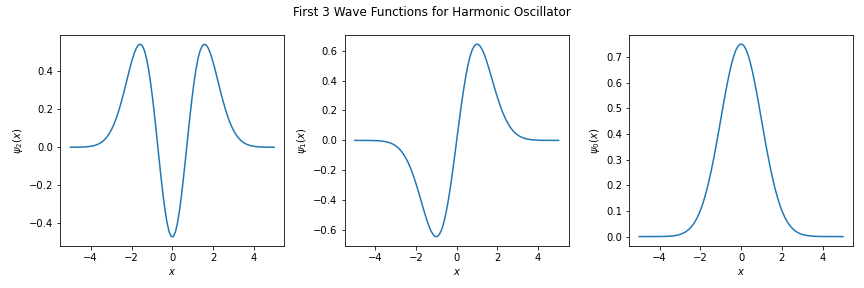
\includegraphics[width=\textwidth]{./chapters/graphs_ch2/2_10_1.png}
}
\exercise{2.11MOD}{
	\begin{itemize}
		\item Compute a general form for $I_s = \int_\mathbb{R} e^{-sx^2}~dx$ for $s >0$. Give an expression for $-\derivative{I_s}{s}$ and also show a general form for its integral over the real numbers. \pagebreak
			\begin{flalign*}
				I_s^2 &= \iint_\mathbb{R} e^{-s(x^2+y^2)}~dx dy\\
				&= \int_{0}^\infty e^{-sr^2} r~dr \int_{0}^{2 \pi} d \theta~~(polar~coord.~transformation)\\
				&= \pi \int_{0}^\infty e^{-st} ~dt~~(substitute~t=r^2)\\
				&= \frac{\pi}{s} \implies I_s = \sqrt{\frac{\pi}{s}}\\
				-\derivative{I_s}{s} &= \int_\mathbb{R} x^2e^{-sx^2}~dx\\
				&= -\derivative{\sqrt{\frac{\pi}{s}}}{s} = \frac{\sqrt{\pi}}{2 s^{3/2}}
			\end{flalign*}
		\item Compute $\langle x \rangle, \langle x^2 \rangle, \langle p \rangle, \langle p^2 \rangle$ for states $\psi_0, \psi_1$ using explicit integration. 
		\begin{flalign*}
			\psi_0(x)&= \Biggl(\frac{m \omega}{\pi \hbar}\Biggr)^{1/4}e^{-\frac{m \omega}{2 \hbar}x^2}\\
			\psi_1(x)&= \Biggl(\frac{m \omega}{\pi \hbar}\Biggr)^{1/4}\sqrt{\frac{2 m \omega }{\hbar}}xe^{-\frac{m \omega}{2 \hbar}x^2}\\\\
			\langle x_0 \rangle &= \int_{\mathbb{R}} \psi_0^*x\psi_0~dx = \sqrt{\frac{m \omega}{\pi \hbar}}\int_{\mathbb{R}} xe^{-\frac{m \omega}{\hbar}x^2}~dx = 0\\
			\langle x_1 \rangle & = \int_{\mathbb{R}} \psi_1^*x\psi_1~dx = \sqrt{\frac{4 m^3 \omega^3}{\pi \hbar^3}}\int_{\mathbb{R}} x^3 e^{-\frac{m \omega}{\hbar}x^2}~dx = 0\\
			\langle x_0^2 \rangle & = \int_{\mathbb{R}} \psi_0^* x^2 \psi_0~dx =  \sqrt{\frac{m \omega}{\pi \hbar}}\int_{\mathbb{R}} x^2 e^{-\frac{m \omega}{\hbar}x^2}~dx\\
			&= \sqrt{\frac{m \omega}{\pi \hbar}} \sqrt{\pi} \frac{1}{2 \frac{m \omega}{\hbar}\sqrt{\frac{m \omega}{\hbar}}}\\
			&= \frac{\hbar}{2 m \omega}\\
			\langle p_0 \rangle &= \int_{\mathbb{R}} \psi_0^* -i\hbar\pdv{}{x} \psi_0~dx = -i\hbar \int_\mathbb{R} \psi_0^* \derivative{\psi_0}{x}~dx\\
			&=i m \omega \sqrt{\frac{m \omega}{\pi \hbar}} \int_\mathbb{R} xe^{-\frac{m \omega}{\hbar}x^2}~dx = 0\\
			\langle p_1 \rangle &= \int_{\mathbb{R}} \psi_1^* -i\hbar\pdv{}{x} \psi_1~dx =-i \hbar \int_\mathbb{R} x(1-\frac{m \omega}{\hbar}x^2)e^{-\frac{m \omega}{\hbar}x^2}~dx = 0\\
			\zeta \equiv \sqrt{\frac{m \omega}{\hbar}}x\\
			\langle x_1^2 \rangle &= \frac{2}{\sqrt{\pi}} \frac{\hbar}{m \omega} \int_{\mathbb{R}} \zeta^4 e^{-\zeta^2} d\zeta\\
			&= \frac{4}{\sqrt{\pi}} \frac{\hbar}{m \omega} \int_0^\infty \zeta^4 e^{-\zeta^2} d\zeta\\
			&= \frac{2}{\sqrt{\pi}} \frac{\hbar}{m \omega} \int_0^\infty u^{3/2}e^{-u} du = \frac{2}{\sqrt{\pi}} \frac{\hbar}{m \omega} \Gamma(5/2)\\
			&= \frac{3 \hbar}{2 m \omega}\\
			\langle p_0^2 \rangle &= -\frac{2 \hbar m \omega}{\sqrt{\pi}}\Biggl(\int_0^\infty \zeta^2 e^{-\zeta^2}~d\zeta - \int_0^\infty e^{-\zeta^2}~d\zeta\Biggr)\\
			&= -\frac{2 \hbar m \omega}{\sqrt{\pi}} \Biggl(\frac{1}{2}\Gamma(5/2)-\sqrt{\pi}\Biggr) = \frac{\hbar m \omega }{2}\\
			\langle p_1^2 \rangle &= \frac{4 \hbar m \omega}{\sqrt{\pi}}\Biggl(3\int_0^\infty \zeta^2 e^{-\zeta^2}~d \zeta - \int_0^\infty \zeta^4 e^{-\zeta^2}~d \zeta\Biggr)\\
			&= \frac{4 \hbar m \omega}{\sqrt{\pi}}\Biggl(\frac{3}{2} \Gamma(3/2) - \frac{1}{2}\Gamma(5/2)\Biggr) = \frac{3 \hbar m \omega}{2}\\
		\end{flalign*}
		\begin{flalign*}
			\sigma_{x_0} &= \sqrt{\frac{\hbar}{2 m \omega}}\\
				\sigma_{p_0} &= \sqrt{\frac{\hbar m \omega}{2}}\\
				\sigma_{x_0}\sigma_{p_0} &= \frac{ \hbar}{2}\\
				\sigma_{x_1} &= \sqrt{\frac{3 \hbar}{2 m \omega}}\\
				\sigma_{p_1} &= \sqrt{\frac{3 \hbar m \omega}{2}}\\
				\sigma_{x_1}\sigma_{p_1} &= \frac{3 \hbar}{2}\\
			\end{flalign*}
			\item Check the uncertainty principle in these cases.
			\begin{flalign*}
				\sigma_{x_0}\sigma_{p_0} &= \frac{\hbar}{2} \geq \frac{\hbar}{2}\\
				\sigma_{x_1}\sigma_{p_1} &= \frac{3 \hbar}{2} \geq \frac{\hbar}{2}
			\end{flalign*}
		\item Compute $\langle T \rangle, \langle V \rangle$ for the states. Is sum what you would expect?
			\begin{flalign*}
				\langle V_0 \rangle &= \langle \frac{m \omega^2 x^2}{2} \rangle = \frac{m \omega^2 \langle x^2 \rangle}{2} = \frac{\hbar \omega }{4}\\
				\langle T_0 \rangle &= \langle \frac{p^2}{2m} \rangle = \frac{\langle p^2 \rangle}{2m} = \frac{\hbar \omega }{4}\\
				\langle T_0 \rangle + \langle V_0 \rangle &= \frac{\hbar}{2}\\
				\langle V_1 \rangle &= \langle \frac{m \omega^2 x^2}{2} \rangle = \frac{m \omega^2 \langle x^2 \rangle}{2} = \frac{3 \hbar \omega }{4}\\
				\langle T_1 \rangle &= \langle \frac{p^2}{2m} \rangle = \frac{\langle p^2 \rangle}{2m} = \frac{3 \hbar \omega }{4}\\
				\langle T_1 \rangle + \langle V_1 \rangle &= \frac{3\hbar}{2}\\
			\end{flalign*}
			We see that the sums are the appropriate energy levels for the ground state and first excited state, respectively.
		\end{itemize}
}

\c{2.12}{
	Compute $\langle x \rangle, \langle x^2 \rangle, \langle p \rangle, \langle p^2 \rangle, \langle T \rangle$ for $n^{th}$ stationary state using ladder operators. 
	\begin{flalign*}
		\langle x \rangle &= \int_\mathbb{R} \psi_n^* \hat{x} \psi_n~dx = \int_\mathbb{R} \psi_n^* \Biggl[\sqrt{\frac{\hbar}{2 m \omega}}(\hat{a}_++\hat{a}_-)\Biggr]\psi_n~dx = \sqrt{\frac{\hbar }{2 m \omega}}\int_\mathbb{R}\psi_n^*(\hat{a}_+\psi_n+\hat{a}_-\psi_n)~dx\\
		&=\sqrt{\frac{\hbar}{2 m \omega}}\int_\mathbb{R}\psi_n^*(A_{n+1}\psi_{n+1}+A_{n-1}\psi_{n-1})~dx\\
		&= \sqrt{\frac{\hbar}{2 m \omega}} \Biggl[A_{n+1}\cancelto{0}{\int_\mathbb{R}\psi_n^*\psi_{n+1}~dx}+A_{n-1}\cancelto{0}{\int_\mathbb{R}\psi_n^*\psi_{n-1}~dx}\Biggr]=0\\
		\langle x^2 \rangle &= \int_\mathbb{R} \psi_n^* \Biggl[\sqrt{\frac{\hbar}{2 m \omega}}(\hat{a}_++\hat{a}_-)\Biggr]^2 \psi_n~dx\\
		&= \frac{\hbar}{2 m \omega}\int_\mathbb{R}\psi_n^*(\hat{a}_+^2+\hat{a}_-\hat{a}_++\hat{a}_+\hat{a}_-+\hat{a}_-^2)\psi_n~dx\\
		&= \frac{\hbar}{2 m \omega}\int_\mathbb{R}\psi_n^* \Biggl[A_{n+2}\psi_{n+2}+n\psi_n+(n+1)\psi_n+A_{n-2}\psi_{n-2}\Biggr]~dx\\
		&= \frac{\hbar}{2 m \omega} \Biggl[  \cancelto{0}{A_{n+2}\int_\mathbb{R} \psi_n^*\psi_{n+2}~dx}+n\cancelto{1}{\int_\mathbb{R}\psi_n^*\psi_n~dx}+(n+1)\cancelto{1}{\int_\mathbb{R}\psi_n^*\psi_n~dx}+A_{n-2}\cancelto{0}{\int_\mathbb{R}\psi_n^*\psi_{n-2}~dx}  \Biggr]\\
		&= \frac{\hbar}{2 m \omega}(2n +1)\\
		\langle p \rangle &= \int_\mathbb{R} \psi_n^*\hat{p}\psi_n~dx = i\sqrt{\frac{\hbar m \omega}{2}}\int_\mathbb{R} \psi_n^* (\hat{a}_+-\hat{a}_-)\psi_n~dx\\
		&= i\sqrt{\frac{\hbar m \omega}{2}}\int_\mathbb{R}\psi_n^*(A_{n+1}\psi_{n+1}-A_{n-1}\psi_{n-1})~dx = 0\\
		\langle p^2 \rangle &= -\frac{\hbar m \omega}{2}\int_\mathbb{R}\psi_n^*(\hat{a}_+^2-\hat{a}_-\hat{a}_+-\hat{a}_+\hat{a}_-+\hat{a}_-^2)\psi_n~dx\\
		&= -\frac{\hbar m \omega}{2}(-(n+1)-n)\\
		&=\frac{\hbar m \omega}{2}(2n+1)\\
		\sigma_x\sigma_p &= \frac{\hbar(2n+1)}{2}\\
		\langle T \rangle &= \frac{\langle p^2 \rangle}{2m} = \frac{\hbar \omega}{4}(2n+1)
	\end{flalign*}
}

\exercise{2.13}{
	A particle in the harmonic oscillator potential starts out in state $$\Psi(x,0)=A\Biggl(3\psi_0(x)+4\psi_1(x)\Biggr)$$
	\begin{itemize}
	\item Find $A$.
		\begin{flalign*}
			1 &= \int_\mathbb{R} \Psi^* \Psi~dx = |A|^2 \int_\mathbb{R} 9\psi_0\psi_0^* + 12 \psi_0\psi_1^* + 12 \psi_1\psi_0^* + 16 \psi_1\psi_1^*~dx\\
			&= A^2\Biggl[9\int_\mathbb{R} \psi_0\psi_0^*~dx+12\int_\mathbb{R} \psi_0\psi_1^*~dx+12\int_\mathbb{R} \psi_1\psi_0^*~dx+16\int_\mathbb{R} \psi_1\psi_1^*~dx\Biggr]\\
			&= 25A^2 \implies A = \frac{1}{5}\\
			\Psi(x,0) = \frac{3}{5}\psi_0 + \frac{4}{5}\psi_1
		\end{flalign*}
   	\item Construct $\Psi(x,t), |\Psi(x,t)|^2$. What would have happened if we specified $\psi_2$ instead of $\psi_1$?
		\begin{flalign*}
			\Psi(x,t)&= \frac{3}{5}\psi_0e^{-i\frac{E_0}{\hbar}t} + \frac{4}{5}\psi_1e^{-i\frac{E_1}{\hbar}t}\\
			&= \frac{3}{5}\Biggl(\frac{m \omega}{\pi \hbar }\Biggr)^{1/4}e^{-\frac{m \omega}{2 \hbar}x^2}e^{i\frac{\omega t}{2}}+\frac{4}{5}\Biggl(\frac{m \omega}{\pi \hbar }\Biggr)^{1/4}xe^{-\frac{3m \omega}{2 \hbar}x^2}e^{-i\frac{3\omega t}{2}}\\
			|\Psi(x,t)|^2 &= \Psi \Psi^* = \frac{1}{25}\sqrt{\frac{m \omega }{\pi \hbar}}\Biggl(\frac{32 m \omega x^2}{\hbar}+24\sqrt{\frac{2 m \omega}{\hbar}}x \cos(\omega t) + 9\Biggr)e^{-\frac{m \omega}{\hbar}x^2}\\
		\end{flalign*}
		The subsitution for the next higher energy state is left as an exercise.
    \item Find $\langle x \rangle, \langle p \rangle$. Check that Ehrenfest's Theorem (Eq. 1.38) holds for this wave function.
		\begin{flalign*}
			\zeta \equiv \sqrt{\frac{m \omega}{\hbar}}x\\
			\langle x \rangle &= \int_\mathbb{R} \Psi^*x\Psi ~dx =  \int_\mathbb{R} x|\Psi|^2~dx = \frac{24}{25}\sqrt{\frac{2}{\pi}}\cos(\omega t)\int_\mathbb{R}\frac{m \omega}{\hbar}x^2e^{-\frac{m \omega}{\hbar}x^2}~dx\\
			&=\frac{48}{25}\sqrt{\frac{2 \hbar}{\pi m \omega}}\cos(\omega t )\cancelto{\frac{1}{2}\Gamma(3/2)}{\int_0^\infty \zeta^2 e^{-\zeta^2}~d\zeta}\\
			&= \frac{12}{25}\sqrt{\frac{2 \hbar}{m \omega}}\cos(\omega t )\\
			\langle p \rangle &= \int_\mathbb{R} \Psi^* -i\hbar \pdv{}{x} \Psi~dx = -i \hbar \int_\mathbb{R} \Psi^* \pdv{\Psi}{x}~dx\\
			&= -\frac{12}{25}\sqrt{2 \hbar m \omega}\sin(\omega t)
		\end{flalign*}
		Confirmation left as an exercise; i.e., $\langle p \rangle = m \langle v \rangle = m \derivative{\langle x \rangle}{t}$; should also see that $\derivative{\langle p \rangle}{t} = \langle -\derivative{V}{x} \rangle$
    \item If you measured the energy of this particle, what values might you get? What are their probabilities?
		\begin{flalign*}
			P_0 &= \Biggl[\frac{3}{5} \Biggr]^2 = 0.36\\
			P_1 &= \Biggl[\frac{4}{5} \Biggr]^2 = 0.64\\
			E_0 &= \frac{\hbar \omega}{2}\\
			E_1 &= \frac{3 \hbar \omega}{2}
		\end{flalign*}
	\end{itemize}
}
\exercise{2.14}{
	In the ground state of the harmonic oscillator, what is the probability (correct to 3 sig figs) of finding the particle outside the classically allowed region?
	Hint: classically, the energy of the oscillator is $E = 0.5kA^2 = 0.5m\omega^2 A^2$ for amplitude $A$. Thus the region is for an energy $E$ extending from $-\sqrt{2E/m\omega^2}$ to $\sqrt{2E/m\omega^2}$. 
	\begin{flalign*}
		\zeta \equiv \sqrt{\frac{m \omega }{\hbar}x}\\
		1 - \int_{-A}^A |\Psi_0(x,t)|^2~dx &= 1 - \int_{-A}^A \psi_0^2~dx = 1 - \sqrt{\frac{m \omega}{\pi \hbar}}\int_{-A}^A e^{-\frac{m \omega}{\hbar}x^2}~dx\\
		&= 1-\frac{2}{\sqrt{\pi}}\int_0^{\sqrt{\frac{m \omega}{\hbar}}A}e^{-\zeta^2}~d\zeta\\
		&= 1 - \erf\Biggl(\sqrt{\frac{m \omega}{\hbar}}A\Biggr)\\
		E_0 &= \frac{\hbar \omega}{2} = \frac{m \omega^2 A^2}{2} \implies A = \sqrt{\frac{\hbar}{m \omega}}\\
		\therefore 1 - P = 1 - \erf(1) \approx 0.157
	\end{flalign*}
}
\exercise{2.15MOD}{
	Use recusion formula (Eq. 2.85) to work out $H_5(\xi)$. Invoke the convention that the highest power of $\xi$ is $2^n$ to fix the overall constant. Then, compute the normalization constant.
	As $n = 5$, we need to set $a_0 = 0$ to kill off even power terms and set $j = 5$ to stop at the proper odd term.
	\begin{flalign*}
		a_{j+2} &= \frac{-2(n-j)}{(j+1)(j+2)}a_j\\
		a_{3} &= \frac{-2(5-1)}{(1+1)(1+2)}a_1 = -\frac{4}{3}a_1\\
		a_{5} &= \frac{-2(5 -3)}{(3+1)(3+2)}a_3 = -\frac{a_3}{5} =  \frac{4}{15}a_1 = 2^5 \implies a_1 = 120\\
		h_5(\xi) &= a_1(\xi - \frac{4}{3}\xi^3 + \frac{4}{15}\xi^5) = 32\xi^5-160\xi^3 +120\xi\\
		\psi_5(\xi) &= h_5(\xi)e^{-\frac{\xi^2}{2}} = 120(\xi - \frac{4}{3}\xi^3 + \frac{4}{15}\xi^5)e^{-\frac{\xi^2}{2}}\\
	\end{flalign*}
	\pagebreak
	Because of the association of the wavefunction with a probability density, it is necessary for the wavefunction to include a normalization constant. We take the moment generating function for the Hermite polynomial and exploit its orthgonality.
	\begin{flalign*}
		\psi_n(\xi)&= c_n H_n(\xi)e^{-\frac{\xi^2}{2}}\\
		g(\xi, z) &= e^{-z^2+2z\xi} = \sum_{n=0}^\infty \frac{z^n}{n!}H_n(\xi)\\
		(First~by~generating~functions)\\
		I &= \int_\mathbb{R} g(\xi,t) e^{-\xi^2/2}g(\xi,s)^*e^{-\xi^2/2}~d\xi\\
		&= e^{st} \int_\mathbb{R} e^{-u^2}~du\\
		&= \sqrt{\pi}e^{2st}\\
		\text(Now~with~Hermite~polynomials)\\
		I &= \int_\mathbb{R} g(\xi,t) e^{-\xi^2/2}g(\xi,s)^*e^{-\xi^2/2}~d\xi\\
		&= \int_\mathbb{R} \sum_{n=0}^\infty \frac{t^n}{n!}H_n(\xi) \sum_{m=0}^\infty \frac{s^m}{m!}H_m(\xi)\\
		&= \sum_{n=0}^\infty \frac{t^n}{n!}\sum_{m=0}^\infty \frac{s^m}{m!}\underbrace{\int_\mathbb{R} H_n(\xi)H_m(\xi)e^{-\xi^2}~d\xi}_{A_{nm}}\\
	\end{flalign*}
	We know the expansion of the Euler constant is $x^n/n!$, so we equate both series as such
	\begin{flalign*}
		\sqrt{\pi} \sum_{n=0}^\infty \frac{(2st)^n}{n!} &= \sum_{n=0}^\infty \frac{t^n}{n!}\sum_{m=0}^\infty \frac{s^m}{m!}A_{nm}\\
		\sqrt{\pi} (2s)^n &= \sum_{m=0}^\infty\frac{s^m}{m!}A_{nm} \implies n = m\\
		\sqrt{\pi} (2)^n &= \frac{1}{n!}A_{nn} \implies \int_\mathbb{R} H_n(\xi)H_m(\xi)e^{-\xi^2}~d\xi = \delta_{nm}\sqrt{\pi}2^n n!\\
		1=\int_\mathbb{R}|\Psi_n|^2~dx &= \int_\mathbb{R} \psi_n^2~dx= c_n^2 \int_\mathbb{R} H_n(\xi)^2e^{-\xi^2}~d\xi = \sqrt{\pi}2^n n!\\
		c_n &= \sqrt{\frac{1}{\sqrt{\pi}2^n n!}}\\
		\therefore \psi_n(\xi) &= \frac{\pi^{-1/4}}{\sqrt{n! 2^n}}H_n(\xi)e^{-\frac{\xi^2}{2}}\\
	\end{flalign*}
	We want a more explicit form in terms of position, so recall $\xi \equiv \sqrt{\frac{m \omega}{\hbar}}x$, which implies $dx = \sqrt{\frac{\hbar}{m \omega}}d\xi$. It follows that
	\begin{flalign*}
		\int_\mathbb{R} H_n(\xi)H_m(\xi)e^{-\xi^2}~d\xi &= \sqrt{\frac{\hbar}{m \omega}}\int_\mathbb{R} H_n(\sqrt{\frac{m \omega}{\hbar}}x)H_m(\sqrt{\frac{m \omega}{\hbar}}x)e^{-\frac{m \omega x^2}{2\hbar}}~dx = \delta_{nm}\sqrt{\pi}2^n n!\\
		\implies c_n &= \Biggl(\frac{m \omega}{\pi \hbar}\Biggr)^{1/4}\frac{1}{\sqrt{2^n n!}}\\
		\therefore \psi_n &= \Biggl(\frac{m \omega}{\pi \hbar}\Biggr)^{1/4}\frac{1}{\sqrt{2^n n!}}H_n(\sqrt{\frac{m \omega}{\hbar}}x)e^{-\frac{m \omega x^2}{2\hbar}}
	\end{flalign*}
}

\exercise{2.16}{
	In this problem we explore some of the more useful theorems (stated without proof) involving Hermite polynomials.
	\begin{itemize}
		\item The Rodrigues forula says that $$h(\xi) = (-1)^n e^{\xi^2}\derivative[n]{}{\xi}e^{-\xi^2}$$ Use it to derive $H_3$ and $H_4$.
			\begin{flalign*}
				H_3(\xi) &= -e^{\xi^2}\derivative[3]{e^{-\xi^2}}{\xi} = 8\xi^3 - 12\xi\\
				H_4(\xi) &= e^{\xi^2}\derivative[4]{e^{-\xi^2}}{\xi} = 16\xi^4-48\xi^2+12\\
			\end{flalign*}
  		\item The following relation gives you $H_{n+1}$ in terms of the preceding Hermite polynomials: $$H_{n+1}(\xi)=2\xi H_n(\xi)-2nH_{n-1}(\xi)$$ Use it, together with previous results, to obtain $H_4$ and $H_5$.
			\begin{flalign*}
				H_{5} &= 2\xi H_{4}-8H_3 = 32\xi^5-160\xi^3+120\xi\\
				H_6 &= 2\xi H_5 - 10H_5 = 64\xi^6-480\xi^4+720\xi^2-120
			\end{flalign*}
    	\item If you differentiate a polynomial of order $n$, you get one of order $n-1$. For Hermite polynomials, $$\derivative{H_n}{\xi}=2nH_{n-1}(\xi)$$ Check this by differentiating $H_5$ and $H_6$.
			\begin{flalign*}
				\derivative{H_5}{\xi} &= \derivative{(32\xi^5 -160\xi^3 +120\xi)}{\xi} = 10(16\xi^4-48\xi^2+12) =10H_4\\
				\derivative{H_6}{\xi} &= \derivative{(64\xi^6-480\xi^5 +720\xi^3 -120)}{\xi} = 12(32\xi^5-160\xi^3+120\xi) =12H_5
			\end{flalign*}
     	\item $H_n(\xi)$ is the $n^{th}$ $z$-derivative, at $z=0$, of the generating function $e^{-z^2+2z\xi}$; or, to put it another way, it's the coefficient $z^n/n!$ in the Taylor series expansion for this function: $$e^{-z^2+2z\xi}=\sum_{n=0}^\infty \frac{z^n}{n!}H_n(\xi)$$ Use this to obtain $H_1$, $H_2$, and $H_3$.
			\begin{flalign*}
				f(z)&=\sum_{n=0}^\infty \frac{f^{(n)}(z_0)}{n!}(z-z_0)^n,~z_0=0\\
				f^{(0)}(z) &= e^{-z^2+2z\xi} &\implies f^{(0)}(0)=1\\
				f^{(1)}(z) &= e^{-z^2+2z\xi}(2\xi-2z) &\implies f^{(1)}(0)=2\xi\\
				f^{(2)}(z) &= e^{-z^2+2z\xi}(2\xi-2z)^2-2e^{-z^2+2z\xi} &\implies f^{(2)}(0)=4\xi^2-2\\
				f^{(3)}(z) &= e^{-z^2+2z\xi}(2\xi-2z)^3-4e^{-z^2+2z\xi}(2\xi-2z)+4e^{-z^2+2z\xi}(z-\xi) &\implies f^{(3)}(0)=8\xi^3-12\xi\\
				\therefore e^{-z^2+2z\xi} &= f^{(0)}(z)+f^{(1)}(z)z+f^{(2)}(z^2)/2!+f^{(3)}(z)/3!+\ldots\\
				&=1+2z\xi+(4\xi^2-2)z^2/2+(8\xi^3-12\xi)z^3/6+\ldots\\
				&= \sum_{n=0}^\infty f^{(n)}(0)\frac{z^n}{n!} \implies f^{(n)}(0) \equiv H_n(\xi)
			\end{flalign*}
	\end{itemize}
}